\documentclass[border=20pt]{standalone}
\usepackage{tikz}
\usepackage{amsmath}
\usetikzlibrary{shapes.geometric, arrows, positioning, decorations.pathreplacing, calc, shapes.symbols}

\definecolor{inputcol}{RGB}{173, 216, 230}
\definecolor{gcncol}{RGB}{144, 238, 144}
\definecolor{poolcol}{RGB}{255, 165, 0}
\definecolor{classcol}{RGB}{221, 160, 221}
\definecolor{outputcol}{RGB}{255, 99, 71}

\begin{document}

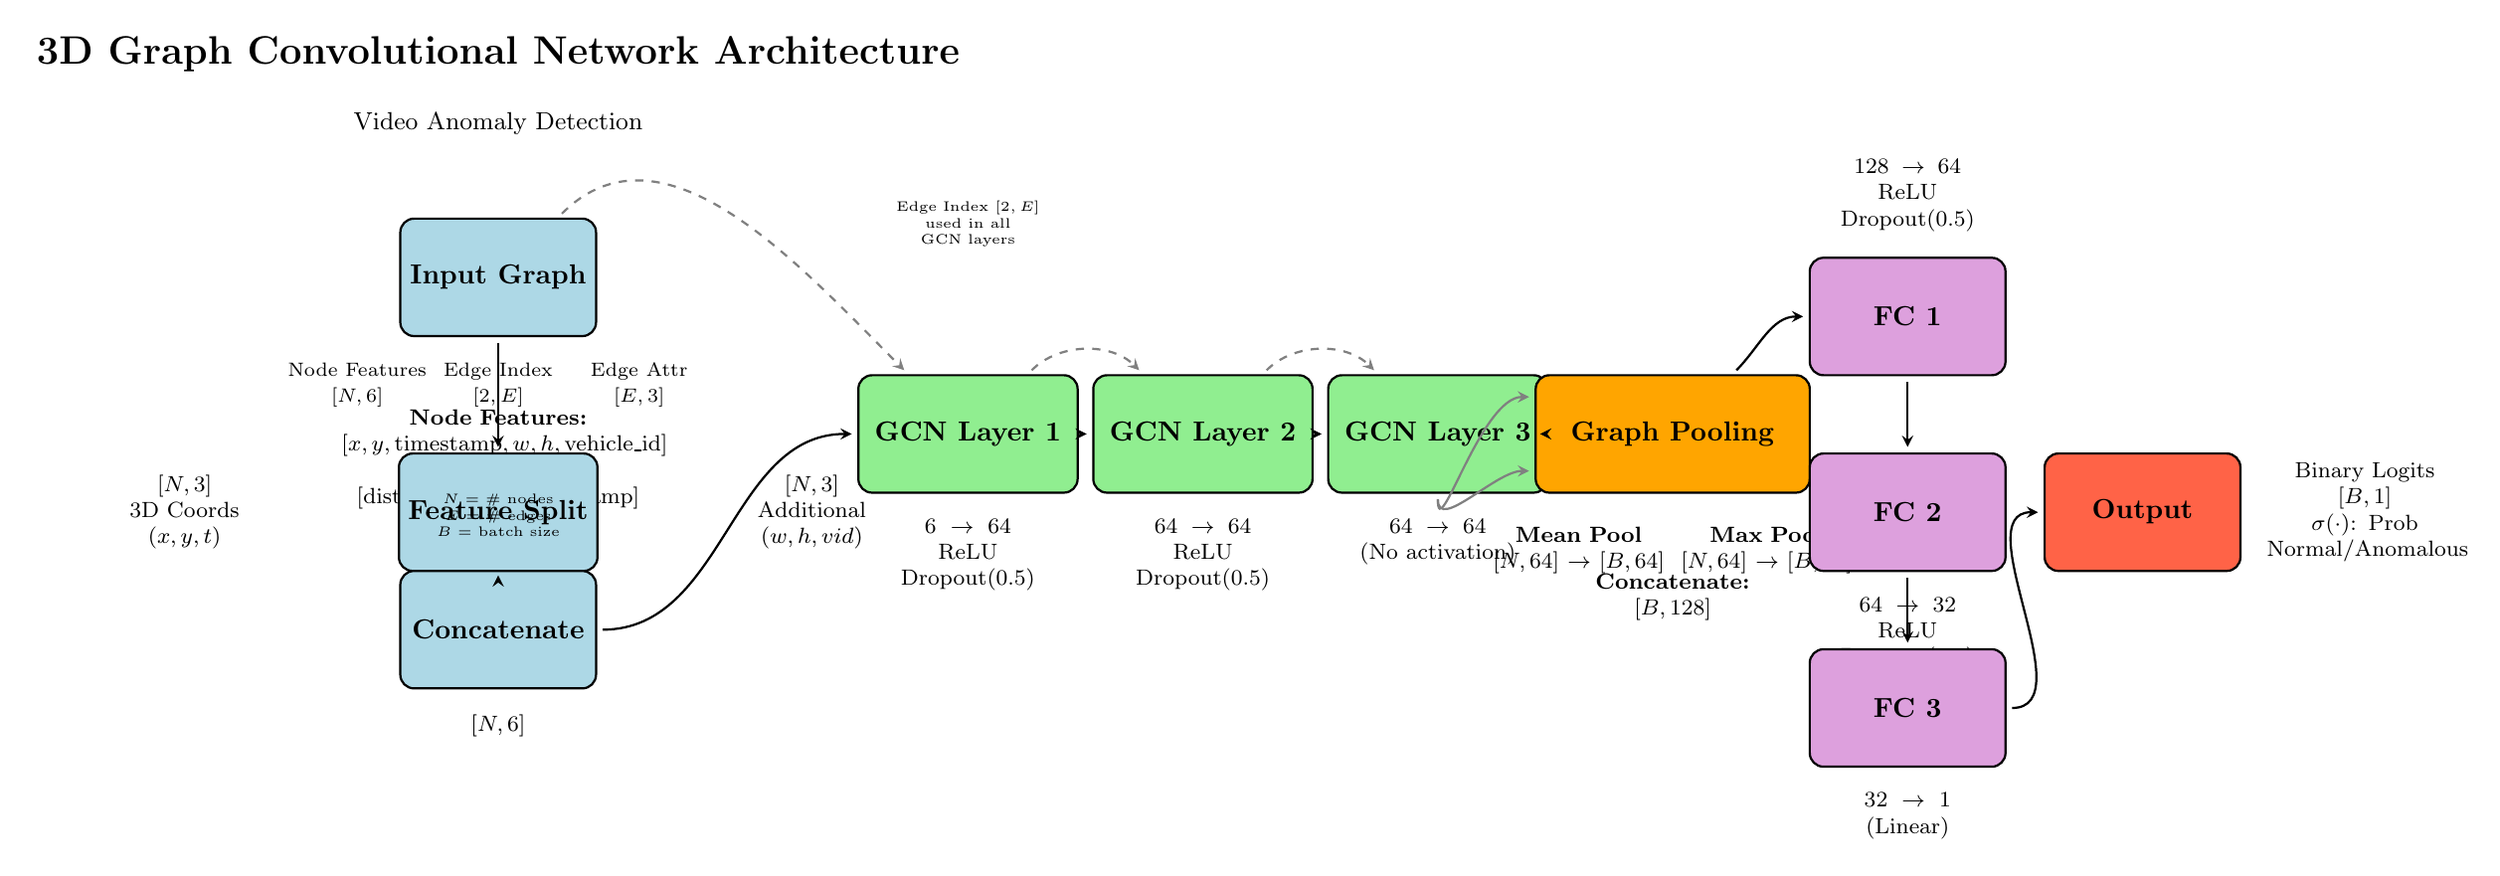
\begin{tikzpicture}[
    node distance = 2cm and 1.5cm,
    box/.style = {rectangle, rounded corners=5pt, minimum width=2.5cm, minimum height=1.5cm, 
                  text centered, draw=black, thick, fill=white},
    input/.style = {box, fill=inputcol},
    gcn/.style = {box, fill=gcncol, minimum width=2.8cm},
    pool/.style = {box, fill=poolcol, minimum width=3.5cm},
    fc/.style = {box, fill=classcol, minimum width=2.5cm},
    output/.style = {box, fill=outputcol},
    arrow/.style = {thick,->,>=stealth, shorten >=2pt, shorten <=2pt},
    dashedarrow/.style = {thick,->,>=stealth, dashed, gray, shorten >=2pt, shorten <=2pt},
    label/.style = {font=\footnotesize, text width=2.5cm, align=center}
]

    % Title
    \node[font=\Large\bfseries, above=0.5cm] at (0,7) {\textbf{3D Graph Convolutional Network Architecture}};
    \node[font=\small, above=0.2cm] at (0,6.5) {Video Anomaly Detection};

    % INPUT LAYER
    \node[input] (input_node) at (0,5) {\textbf{Input Graph}};
    \node[label, below=0.2cm of input_node, xshift=-1.8cm] {\scriptsize Node Features\\\scriptsize $[N, 6]$};
    \node[label, below=0.2cm of input_node] {\scriptsize Edge Index\\\scriptsize $[2, E]$};
    \node[label, below=0.2cm of input_node, xshift=1.8cm] {\scriptsize Edge Attr\\\scriptsize $[E, 3]$};
    
    \node[label, below=0.8cm of input_node, text width=4cm] {
        \textbf{Node Features:}\\
        $[x, y, \text{timestamp}, w, h, \text{vehicle\_id}]$\\
        \textbf{Edge Features:}\\
        $[\text{distance}, \text{frame}, \text{timestamp}]$
    };

    % FEATURE PROCESSING
    \node[input] (split) at (0,2) {\textbf{Feature Split}};
    \node[label, left=0.3cm of split, xshift=-1.2cm, text width=2.2cm] {
        $[N, 3]$\\
        3D Coords\\
        $(x, y, t)$
    };
    \node[label, right=0.3cm of split, xshift=1.2cm, text width=2.2cm] {
        $[N, 3]$\\
        Additional\\
        $(w, h, vid)$
    };

    \node[input] (concat) at (0,0.5) {\textbf{Concatenate}};
    \node[label, below=0.2cm of concat] {$[N, 6]$};

    % GCN LAYERS
    \node[gcn] (gcn1) at (6,3) {\textbf{GCN Layer 1}};
    \node[label, below=0.2cm of gcn1] {
        $6 \to 64$\\
        ReLU\\
        Dropout(0.5)
    };

    \node[gcn] (gcn2) at (9,3) {\textbf{GCN Layer 2}};
    \node[label, below=0.2cm of gcn2] {
        $64 \to 64$\\
        ReLU\\
        Dropout(0.5)
    };

    \node[gcn] (gcn3) at (12,3) {\textbf{GCN Layer 3}};
    \node[label, below=0.2cm of gcn3] {
        $64 \to 64$\\
        (No activation)
    };

    % GRAPH POOLING
    \node[pool] (pool) at (15,3) {\textbf{Graph Pooling}};
    \node[label, below=0.3cm of pool, xshift=-1.2cm, text width=2.5cm] {
        \textbf{Mean Pool}\\
        $[N, 64] \to [B, 64]$
    };
    \node[label, below=0.3cm of pool, xshift=1.2cm, text width=2.5cm] {
        \textbf{Max Pool}\\
        $[N, 64] \to [B, 64]$
    };
    \node[label, below=0.9cm of pool] {
        \textbf{Concatenate:} $[B, 128]$
    };

    % CLASSIFIER
    \node[fc] (fc1) at (18,4.5) {\textbf{FC 1}};
    \node[label, above=0.2cm of fc1] {
        $128 \to 64$\\
        ReLU\\
        Dropout(0.5)
    };

    \node[fc] (fc2) at (18,2) {\textbf{FC 2}};
    \node[label, below=0.2cm of fc2] {
        $64 \to 32$\\
        ReLU\\
        Dropout(0.5)
    };

    \node[fc] (fc3) at (18,-0.5) {\textbf{FC 3}};
    \node[label, below=0.2cm of fc3] {
        $32 \to 1$\\
        (Linear)
    };

    % OUTPUT
    \node[output] (output) at (21,2) {\textbf{Output}};
    \node[label, right=0.2cm of output, text width=2.5cm] {
        Binary Logits\\
        $[B, 1]$\\
        $\sigma(\cdot)$: Prob\\
        Normal/Anomalous
    };

    % ARROWS - Main flow
    \draw[arrow] (input_node) to[out=270, in=90] (split);
    \draw[arrow] (split) -- (concat);
    \draw[arrow] (concat) to[out=0, in=180] (gcn1);
    \draw[arrow] (gcn1) -- (gcn2);
    \draw[arrow] (gcn2) -- (gcn3);
    \draw[arrow] (gcn3) -- (pool);
    \draw[arrow] (pool) to[out=45, in=180] (fc1);
    \draw[arrow] (fc1) -- (fc2);
    \draw[arrow] (fc2) -- (fc3);
    \draw[arrow] (fc3) to[out=0, in=180] (output);

    % Edge index flow (dashed)
    \draw[dashedarrow] (input_node) to[out=45, in=135] (gcn1);
    \draw[dashedarrow] (gcn1) to[out=45, in=135] (gcn2);
    \draw[dashedarrow] (gcn2) to[out=45, in=135] (gcn3);
    
    % Pooling branches
    \draw[arrow, gray] (gcn3) to[out=270, in=180] (pool.195);
    \draw[arrow, gray] (gcn3) to[out=270, in=180] (pool.165);

    % Batch vector annotation
    \node[label, above=1.5cm of gcn1, text width=3cm, font=\tiny] {
        Edge Index $[2, E]$\\
        used in all\\
        GCN layers
    };

    % Dimension annotations
    \node[label, above=0.3cm of concat, text width=3cm, font=\tiny] {
        $N$ = \# nodes\\
        $E$ = \# edges\\
        $B$ = batch size
    };

\end{tikzpicture}

\end{document}

